\documentclass[a4paper,german,12pt,smallheadings]{scrartcl}
\usepackage[T1]{fontenc}
\usepackage[utf8]{inputenc}
\usepackage{babel}
\usepackage{geometry}
\usepackage{pdfpages}
\usepackage{tikz}
\usepackage{wrapfig}
\usepackage[fleqn]{amsmath}
\usepackage{amssymb}
\usepackage{float}
\usepackage{enumerate}
\usepackage{listings} % Source code
\usepackage{lscape} % landscape
\usepackage{commath} % http://tex.stackexchange.com/questions/14821/whats-the-proper-way-to-typeset-a-differential-operator
\usepackage{cancel}
\usepackage[fleqn]{mathtools}
% Number only referenced equations
%\mathtoolsset{showonlyrefs}

%\usepackage{wrapfig}
\usepackage{siunitx}
\sisetup{separate-uncertainty=true,locale=DE}

% New command for color underlining
\usepackage{xcolor}
\newcommand\invisiblesection[1]{%
    \refstepcounter{section}%
      \addcontentsline{toc}{section}{\protect\numberline{\thesection}#1}%
        \sectionmark{#1}}
\newsavebox\MBox
\newcommand\colul[2][red]{{\sbox\MBox{$#2$}%
  \rlap{\usebox\MBox}\color{#1}\rule[-1.2\dp\MBox]{\wd\MBox}{0.5pt}}}

\restylefloat{table}
\geometry{a4paper, top=15mm, left=20mm, right=10mm, bottom=20mm, headsep=10mm, footskip=12mm}
\linespread{1.5}
\setlength\parindent{0pt}
\DeclareMathOperator{\Tr}{Tr}
\DeclareMathOperator{\Var}{Var}
\begin{document}

\begin{titlepage}
\newcommand{\HRule}{\rule{\linewidth}{0.5mm}}

\begin{center}
  \textsc{\Large Physikalisches Grundpraktkum 1}
  \HRule\\[0.4 cm]
  {\huge \bfseries Gleichmäßig beschleunigte Drehbewegungen}
  \HRule\\[0.4 cm]

  \begin{minipage}{0.65\textwidth}
  \begin{flushleft}
    Markus Fenske \texttt{<iblue@zedat.fu-berlin.de>} \\
    Paul Rahmann \texttt{<paulrahmann@zedat.fu-berlin.de>}
  \end{flushleft}
  \end{minipage}
  \hfill
  \begin{minipage}{0.30\textwidth}
  \begin{flushright}
    Tutor: Christian Hindermann \\
    Versuchstag: 6. Juni 2014
  \end{flushright}
  \end{minipage}

  \vspace{1cm}

  \tableofcontents


  %{\large \today}
  \vfill
\end{center}
\newpage

\end{titlepage}

\allowdisplaybreaks % Seitenumbrüche in Formeln erlauben
\begin{center}
\bfseries % Fettdruck einschalten
\sffamily % Serifenlose Schrift
\vspace{-40pt}
Physikalisches Grundpraktikum 2, Wintersemester 2014/2015

Markus Fenske \texttt{<iblue@zedat.fu-berlin.de>}

Alexandra Krause \texttt{<alexandra.krause2@gmail.com>}

Mikroskop, Tutor: Kevin Madsen
\vspace{-10pt}
\end{center}

\section{Physikalische Grundlagen}

Das menschliche Auge ist in der Lage Gegenstände ab einer Größe von $0{,}02
\operatorname{mm}$ zu betrachten. Um kleinere Gegenstände wahrzunehmen, werden
optische Hilfsmittel wie Lupe oder Mikroskop benötigt. Diese sollen im
Folgenden untersucht werden.

\subsection{Geometrische Optik}

Die Physik kennt viele verschiedene Beschreibungen der elektromagnetischen
Wellen. Für den Spezialfall des Lichtes in der Optik besonders geeignet ist die
\textit{Geometrische Optik}. Dabei wird die Wellen- und Teilchennatur des
Lichtes vernachlässigt und vereinfachend angenommen, das Licht bestünde aus
Lichtstrahlen, die sich geradlinig fortbewegen und ihre Richtung nur an
jeweiligen Brechkanten gemäß des Snelliusschen Brechnungsgesetzes ändern (siehe
vorheriger Versuch).

\subsection{Dünne Linsen}

\begin{figure}[h]
  \centering
  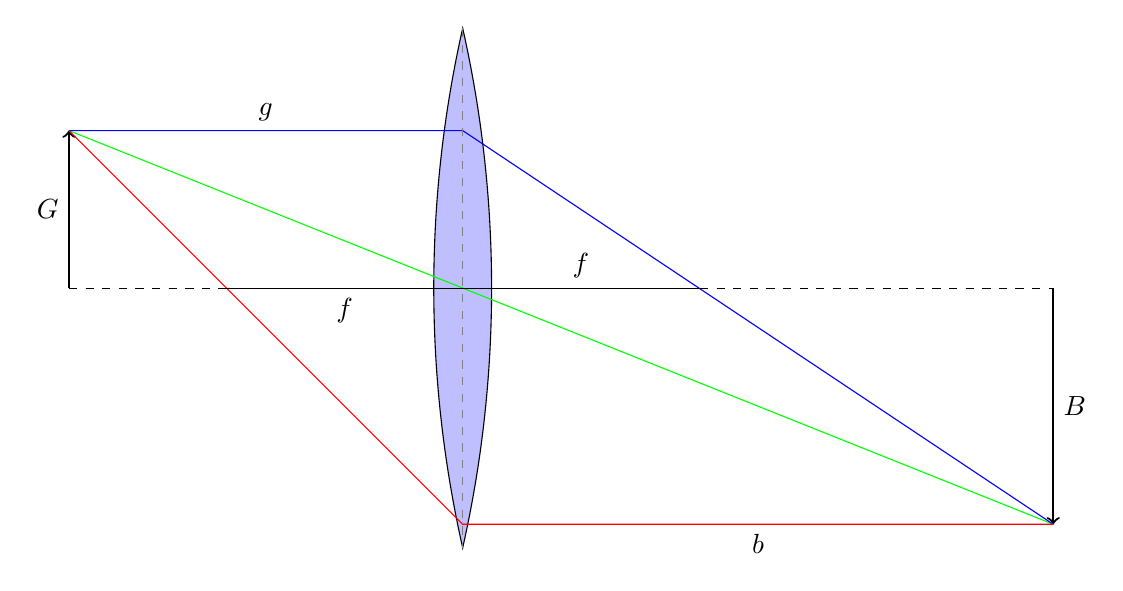
\begin{tikzpicture}
    \pgfmathsetmacro{\lensRadius}{15}
    \pgfmathsetmacro{\lensHeight}{3.3}
    \pgfmathsetmacro{\startAngle}{asin(\lensHeight/\lensRadius)}
    \pgfmathsetmacro{\focalLength}{3}
    \pgfmathsetmacro{\objectDistance}{5}
    \pgfmathsetmacro{\objectHeight}{2}
    \pgfmathsetmacro{\pictureDistance}{1/((1/\focalLength)-(1/\objectDistance))}
    \pgfmathsetmacro{\pictureHeight}{\pictureDistance/\objectDistance*\objectHeight}

    % Linse
    \draw [fill=blue!25]  (0,\lensHeight)
    arc[start angle=180-\startAngle,delta angle=2*\startAngle,radius=\lensRadius]
    arc[start angle=-\startAngle,delta angle=2*\startAngle,radius=\lensRadius]
     -- cycle;

    % Gegenstand
    \draw[thick,->] (-\objectDistance,0) -- node[left] {$G$} (-\objectDistance,\objectHeight);

    % Bild
    \draw[thick,->] (\pictureDistance,0) -- node[right] {$B$} (\pictureDistance,-\pictureHeight);

    % Mittelpunktstrahl
    \draw[color=green] (-\objectDistance,\objectHeight) -- (\pictureDistance,-\pictureHeight);

    % Parallelstrahl
    \draw[color=blue] (-\objectDistance,\objectHeight) -- node[above,color=black] {$g$} (0,\objectHeight) -- (\pictureDistance,-\pictureHeight);

    % Brennpunktstrahl
    \draw[color=red] (-\objectDistance,\objectHeight) -- (0,-\pictureHeight) -- node[below,color=black] {$b$} (\pictureDistance,-\pictureHeight);

    % Optische Achse
    \draw[dashed] (-\objectDistance,0) -- (\pictureDistance,0);

    % Brennweite
    \draw (-\focalLength,0) -- node[below] {$f$} (0,0);
    \draw (0,0) -- node[above] {$f$} (\focalLength,0);

    % Vertikale Achse
    \draw[dashed,gray] (0,\lensHeight) -- (0,-\lensHeight);
  \end{tikzpicture}
  \caption{Strahlengang}
  \label{fig:rays}
\end{figure}

Besonders wichtig für diesen Versuch ist dabei die Beschreibung von
Sammellinsen. Sammellinsen sind in erster Näherung Glaskörper in der Form der
Schnittmenge zweier gleich großer Vollkugeln. Interessant ist, in welcher Art
sich nun Lichtstrahlen durch Sammellinsen bewegen. Man stellt fest, dass für
den Spezialfall, dass die Linse klein gegenüber dem Radius der begrenzenden
Vollkugeln sind, es drei Arten von Strahlen gibt, die sich gegenüber den
anderen auszeichnen:

\begin{itemize}
  \item Der \textit{Mittelpunktstrahl} (in der Abbildung grün) durchläuft die
    Linse ohne durch Brechnung abgelenkt zu werden.
  \item Der \textit{Parallelstrahl} (in der Abbildung blau) trifft parallel zur
    optischen Achse (also der Achse durch den Mittelpunkt der beiden gedachten
    Vollkugeln) auf die Linse. Er wird immer derart gebrochen, dass er durch
    einen Punkt geht, den wir im folgenden als \textit{Brennpunkt} $F$
    bezeichnen wollen.
  \item Da es sich um eine bijektive Abbildung handelt, wird jeder Strahl, der
    durch den Brennpunkt geht, wieder zum Parallelstrahl. Diesen nennen wir
    \textit{Brennpunktstrahl} (in der Abbildung rot).
\end{itemize}

Abbildung \ref{fig:rays} gibt unter Verwendung dieser Definitionen den Strahlengang durch
eine dünne Linse an.

Damit lässt sich nun die Abbildungsgleichung herleiten.

\begin{figure}[h]
  \centering
  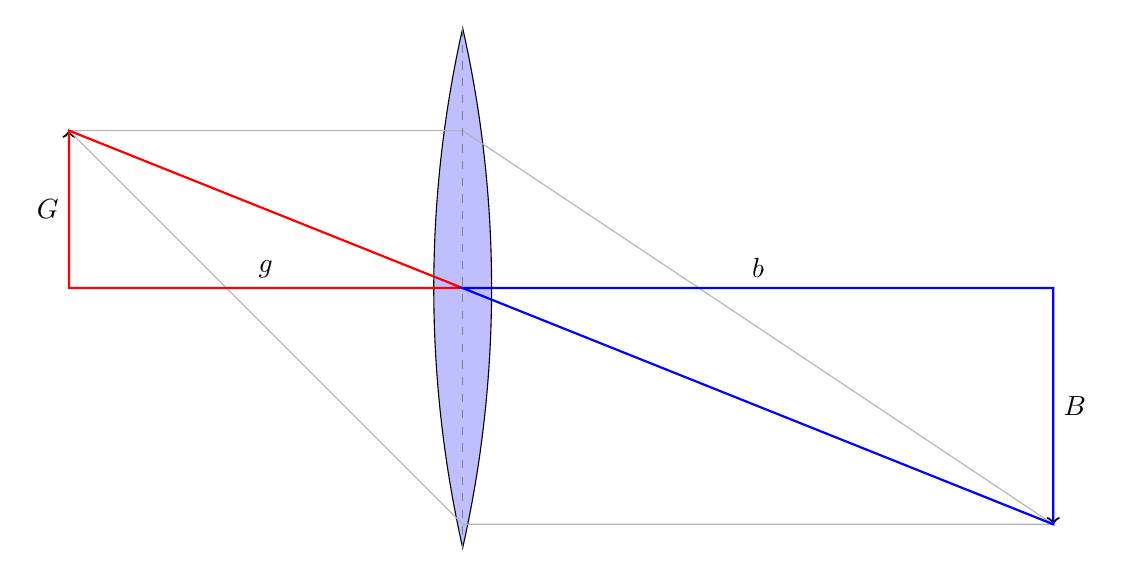
\begin{tikzpicture}
    \pgfmathsetmacro{\lensRadius}{15}
    \pgfmathsetmacro{\lensHeight}{3.3}
    \pgfmathsetmacro{\startAngle}{asin(\lensHeight/\lensRadius)}
    \pgfmathsetmacro{\focalLength}{3}
    \pgfmathsetmacro{\objectDistance}{5}
    \pgfmathsetmacro{\objectHeight}{2}
    \pgfmathsetmacro{\pictureDistance}{1/((1/\focalLength)-(1/\objectDistance))}
    \pgfmathsetmacro{\pictureHeight}{\pictureDistance/\objectDistance*\objectHeight}

    % Linse
    \draw [fill=blue!25]  (0,\lensHeight)
    arc[start angle=180-\startAngle,delta angle=2*\startAngle,radius=\lensRadius]
    arc[start angle=-\startAngle,delta angle=2*\startAngle,radius=\lensRadius]
     -- cycle;

    % Gegenstand
    \draw[thick,->] (-\objectDistance,0) -- node[left] {$G$} (-\objectDistance,\objectHeight);

    % Bild
    \draw[thick,->] (\pictureDistance,0) -- node[right] {$B$} (\pictureDistance,-\pictureHeight);

    % Mittelpunktstrahl
    %\draw (-\objectDistance,\objectHeight) -- (\pictureDistance,-\pictureHeight);

    % Parallelstrahl
    \draw[color=gray!60] (-\objectDistance,\objectHeight) -- (0,\objectHeight) -- (\pictureDistance,-\pictureHeight);

    % Brennpunktstrahl
    \draw[color=gray!60] (-\objectDistance,\objectHeight) -- (0,-\pictureHeight) -- (\pictureDistance,-\pictureHeight);

    % Optische Achse
    \draw[dashed] (-\objectDistance,0) -- (\pictureDistance,0);

    % Brennweite
    %\draw (-\focalLength,0) -- node[below] {f} (0,0);
    %\draw (0,0) -- node[above] {f} (\focalLength,0);

    % Vertikale Achse
    \draw[dashed,gray] (0,\lensHeight) -- (0,-\lensHeight);

    % Hervorrhebung
    \draw[thick,color=red] (0,0) -- (-\objectDistance,\objectHeight) -- (-\objectDistance,0) -- node[above,color=black] {$g$} cycle;
    \draw[thick,color=blue] (0,0) -- (\pictureDistance,-\pictureHeight) -- (\pictureDistance,0) -- node[above,color=black] {$b$} cycle;
  \end{tikzpicture}
  \caption{Zur Herleitung, Teil 1}
  \label{fig:eq1}
\end{figure}

Die Dreiecke, bestehend aus den Strecken $G$, $g$ und dem halben
Mittelpunktstrahl und aus $B$, $b$ und dem halben Mittelpunktstrahl, sind
ähnlich, denn sie stimmen in allen Winkeln überein (rechter Winkel zwischen $G$
und $g$ sowie $B$ und $b$ und Wechselwinkel am Mittelpunktstrahl). Somit müssen
die Streckenverhältnisse gleich sein (siehe Abbildung \ref{fig:eq1}). Wir
definieren darüber den Abbildungsmaßstab $\beta$.

\begin{equation}
  \beta = \frac{B}{G} = \frac{b}{g}
  \label{eq:beta}
\end{equation}

\begin{figure}[h]
  \centering
  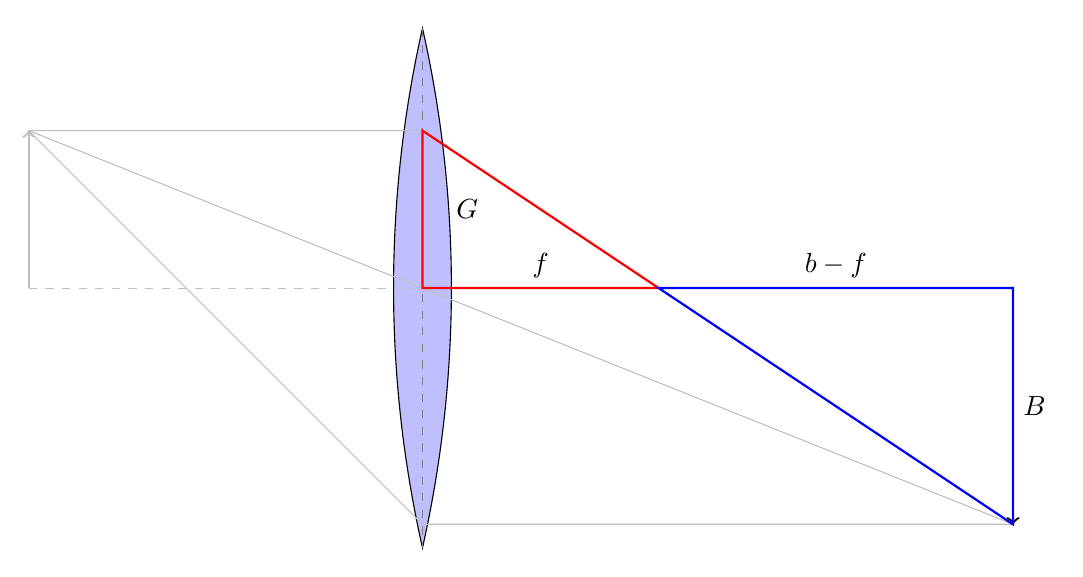
\begin{tikzpicture}
    \pgfmathsetmacro{\lensRadius}{15}
    \pgfmathsetmacro{\lensHeight}{3.3}
    \pgfmathsetmacro{\startAngle}{asin(\lensHeight/\lensRadius)}
    \pgfmathsetmacro{\focalLength}{3}
    \pgfmathsetmacro{\objectDistance}{5}
    \pgfmathsetmacro{\objectHeight}{2}
    \pgfmathsetmacro{\pictureDistance}{1/((1/\focalLength)-(1/\objectDistance))}
    \pgfmathsetmacro{\pictureHeight}{\pictureDistance/\objectDistance*\objectHeight}

    % Linse
    \draw [fill=blue!25]  (0,\lensHeight)
    arc[start angle=180-\startAngle,delta angle=2*\startAngle,radius=\lensRadius]
    arc[start angle=-\startAngle,delta angle=2*\startAngle,radius=\lensRadius]
     -- cycle;

    % Gegenstand
    \draw[thick,->,gray!50] (-\objectDistance,0) -- (-\objectDistance,\objectHeight);

    % Bild
    \draw[thick,->] (\pictureDistance,0) -- node[right] {$B$} (\pictureDistance,-\pictureHeight);

    % Mittelpunktstrahl
    \draw[gray!50] (-\objectDistance,\objectHeight) -- (\pictureDistance,-\pictureHeight);

    % Parallelstrahl
    \draw[gray!50] (-\objectDistance,\objectHeight) -- (0,\objectHeight) -- (\pictureDistance,-\pictureHeight);

    % Brennpunktstrahl
    \draw[gray!50] (-\objectDistance,\objectHeight) -- (0,-\pictureHeight) -- (\pictureDistance,-\pictureHeight);

    % Optische Achse
    \draw[dashed,gray!50] (-\objectDistance,0) -- (\pictureDistance,0);

    % Vertikale Achse
    \draw[dashed,gray] (0,\lensHeight) -- (0,-\lensHeight);

    % Hervorrhebung
    \draw[thick,color=red] (0,0) -- node[color=black,right=0.3cm] {$G$} (0,\objectHeight) -- (\focalLength,0) -- node[color=black,above] {$f$} cycle;
    \draw[thick,color=blue] (\focalLength,0) -- (\pictureDistance,-\pictureHeight) -- (\pictureDistance,0) -- node[above,color=black] {$b - f$} cycle;
  \end{tikzpicture}
  \caption{Zur Herleitung, Teil 2}
  \label{fig:eq2}
\end{figure}

Auf der Seite des Bildes wird ein Dreieck gebildet aus der der Strecke
$f$, der Gegenstandshöhe $G$ in der Linsenebene und dem halben
Brennpunktstrahl. Das Dreieck aus $B$, $b-f$ und der anderen Hälfte des
Brennpunktstrahls ist dazu aus den selben Gründen wie oben ähnlich (siehe
Abbildung \ref{fig:eq2}). Somit gilt

\begin{equation*}
  \frac{B}{G} = \frac{b-f}{f}
\end{equation*}

Zusammengesetzt ergibt sich
\begin{equation}
  \frac{b}{g} = \frac{b-f}{f}
  \label{eq:inter}
\end{equation}

Durch Division durch $b$ und Addition von $\frac{1}{b}$ erhält man die
Abbildungsgleichung

\begin{equation}
  \frac{1}{f} = \frac{1}{b} + \frac{1}{g}
\end{equation}

% Aufgabe 2
% http://www.wolframalpha.com/input/?i=solve+1%2Ff+%3D+1%2Fg+%2B+1%2F%28e-g%29+for+g
Um bei einem festen Abstand $e = g+b$ zwischen Gegenstand und Bild ein scharfes
Bild zu erhalten, gibt es genau zwei Möglichkeiten. Dies sieht man durch
Einsetzen in die Linsengleichung und Umstellen. Mittels Computeralgebrasystem
ergeben sich die zwei Lösungen

\begin{equation}
  g = \pm \frac{1}{2} \del{\sqrt{e^2 - 4ef} + e}
\end{equation}

% FIXME: Warum? beta = (e-g)/g für beide Lösungen ausrechnen!
Dabei handelt es sich einmal um eine Vergrößerung ($\beta > 1$) und einmal um
eine Verkleinerung ($\beta < 1$).


\subsection{Dicke Linsen}

Die idealisierte Vorstellung einer dünnen Linse gilt nur in erster Näherung.
Der Realität näher kommt das Modell der dicken Linse. Dabei wird das System
zusätzlich durch die beiden Hauptebenen bestimmt. Die beiden Hauptebenen sind
dabei durch einen Abstand $i$ entfernt. Die nachfolgende Abbildung
\ref{fig:thicklens} verdeutlicht das Modell anhand des Strahlengangs.

\begin{figure}[h]
  \centering
  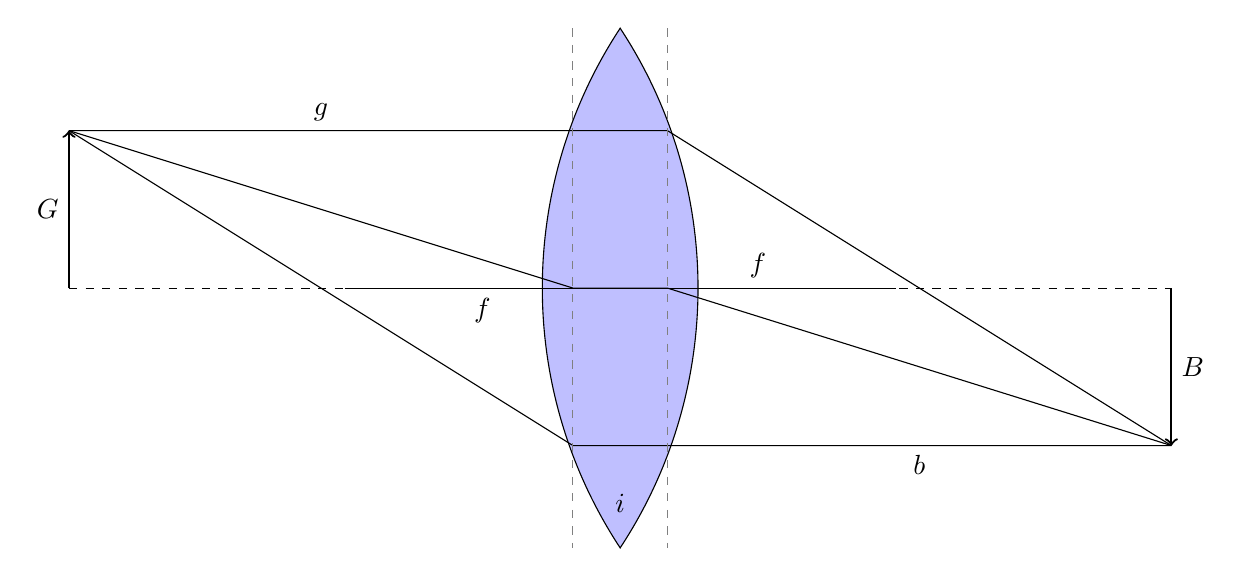
\begin{tikzpicture}
    \pgfmathsetmacro{\lensRadius}{6}
    \pgfmathsetmacro{\lensHeight}{3.3}
    \pgfmathsetmacro{\startAngle}{asin(\lensHeight/\lensRadius)}
    \pgfmathsetmacro{\focalLength}{3.5}
    \pgfmathsetmacro{\focalDistance}{0.6}
    \pgfmathsetmacro{\objectDistance}{7}
    \pgfmathsetmacro{\objectHeight}{2}
    \pgfmathsetmacro{\pictureDistance}{1/((1/\focalLength)-(1/\objectDistance))}
    \pgfmathsetmacro{\pictureHeight}{\pictureDistance/\objectDistance*\objectHeight}

    % Linse
    \draw [fill=blue!25]  (0,\lensHeight)
    arc[start angle=180-\startAngle,delta angle=2*\startAngle,radius=\lensRadius]
    arc[start angle=-\startAngle,delta angle=2*\startAngle,radius=\lensRadius]
     -- cycle;

    % Gegenstand
    \draw[thick,->] (-\objectDistance,0) -- node[left] {$G$} (-\objectDistance,\objectHeight);

    % Bild
    \draw[thick,->] (\pictureDistance,0) -- node[right] {$B$} (\pictureDistance,-\pictureHeight);

    % Mittelpunktstrahl
    \draw (-\objectDistance,\objectHeight) -- (-\focalDistance,0) -- (\focalDistance,0) -- (\pictureDistance,-\pictureHeight);

    % Parallelstrahl
    \draw (-\objectDistance,\objectHeight) -- node[above,color=black] {$g$} (-\focalDistance,\objectHeight) -- (\focalDistance,\objectHeight)  --(\pictureDistance,-\pictureHeight);

    % Brennpunktstrahl
    \draw (-\objectDistance,\objectHeight) -- (-\focalDistance,-\pictureHeight) -- node[below=0.5cm,color=black] {$i$}  (\focalDistance,-\pictureHeight) -- node[below,color=black] {$b$} (\pictureDistance,-\pictureHeight);

    % Optische Achse
    \draw[dashed] (-\objectDistance,0) -- (\pictureDistance,0);

    % Brennweite
    \draw (-\focalLength,0) -- node[below] {$f$} (0,0);
    \draw (0,0) -- node[above] {$f$} (\focalLength,0);

    % Vertikale Achse
    \draw[dashed,gray] (-\focalDistance,\lensHeight) -- (-\focalDistance,-\lensHeight);
    \draw[dashed,gray] (\focalDistance,\lensHeight) -- (\focalDistance,-\lensHeight);
  \end{tikzpicture}
  \caption{Strahlengang einer dicken Linse}
  \label{fig:thicklens}
\end{figure}


% Aufgabe 3
Die geometrischen Überlegungen gelten genauso für dicke Linsen, denn schneidet
man die Hauptebenen heraus, ergeben sich die selben geometrischen
Zusammenhänge. Problematisch ist nur, dass sich aufgrund des unbekannten
Hauptebenenabstands die Gegenstands- und die Bildweite nicht mehr bestimmen
lassen. Der Brennwert muss sich also aus einem anderen Zusammenhang ergeben.
Messbar sind $g-b$ und $\beta$, so dass daraus der Brennwert berechnet werden
muss.

Durch Einsetzen von (\ref{eq:beta}) in (\ref{eq:inter}) erhalten wir

\begin{equation}
  \beta = \frac{b-f}{f}
\end{equation}

Umgestellt nach $f$:
\begin{equation}
  f = \frac{b}{\beta + 1}
\end{equation}

Durch Erweitern mit $\beta - 1$:
\begin{equation}
  f = \frac{b(\beta - 1)}{1-\beta^2}
\end{equation}

Durch Erweitern mit $\frac{1}{\beta} = \frac{g}{b}$:

\begin{equation}
  f = \frac{g - b}{\frac{1}{\beta} - \beta}
  \label{eq:dickebrennweite}
\end{equation}

Somit ist die Brennweite nur durch $g-b$ und $\beta$ ausgedrückt.

Aus $e = g + i + b$ erhalten wir

\begin{align*}
  i &= e - (g+b) \\
    &= e - (g-b) \frac{g+b}{g-b} \\
    &= e - (g-b) \frac{(g+b)\beta}{(g-b)\beta} \\
    &= e - (g-b) \frac{b + \beta b}{b - \beta b} \\
    &= e - (g-b) \frac{\beta + 1}{\beta - 1}
\end{align*}

\subsection{Mikroskop}
Um eine Vergrößerung eines realen Gegenstands zu erreichen, verwendet man oft
ein System aus zwei Sammellinsen, genannt Mikroskop. Dabei wird zuerst mit der
ersten Linse (Objektiv) ein reelles Zwischenbild des Gegenstands erzeugt, dass
dann mit einem als Lupe wirkenden Okular betrachtet wird.

% Aufgabe 4: Zeug malen (Aus Skript übernehmen?)
\begin{figure}[h!]
    \centering
    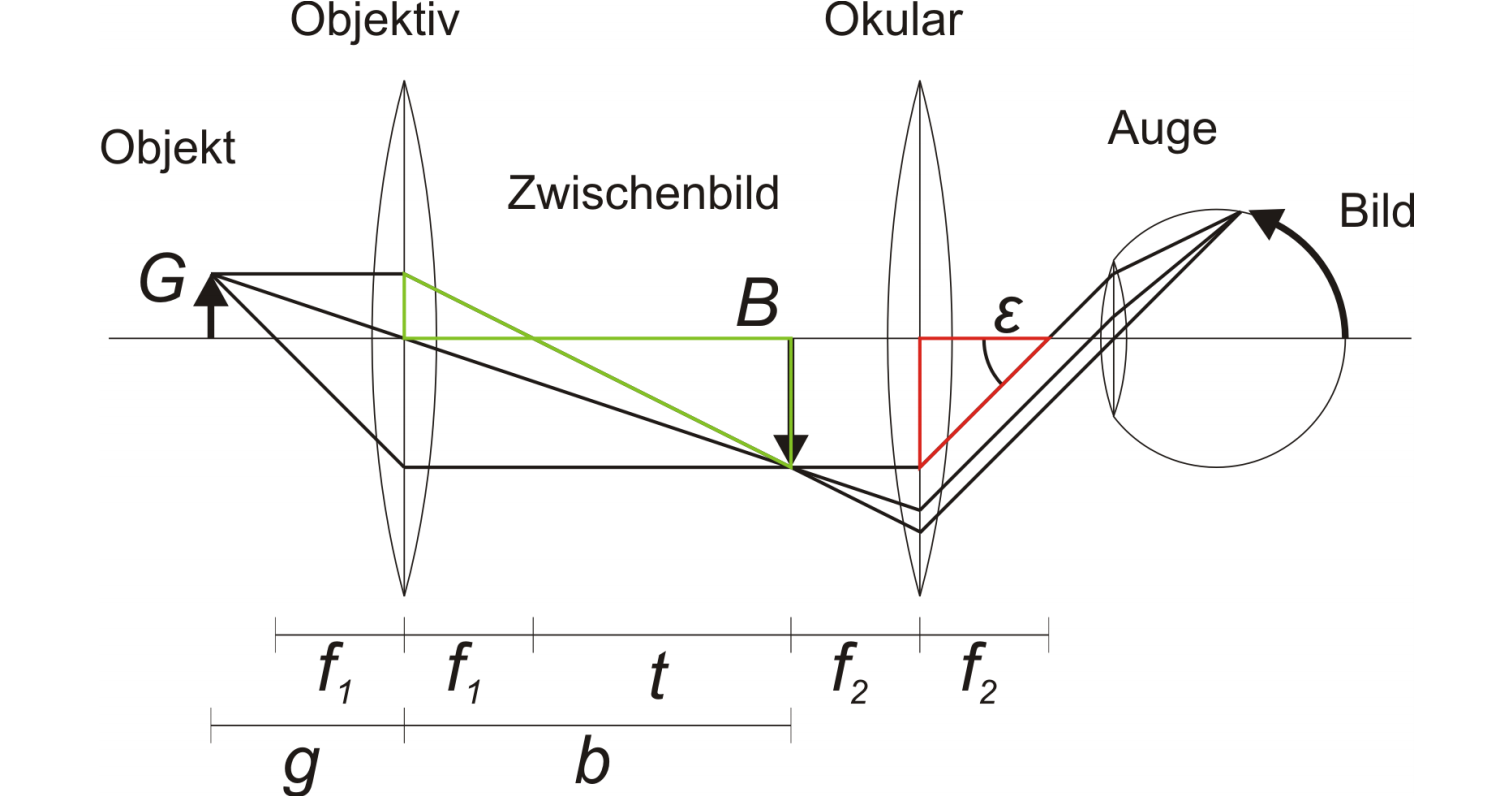
\includegraphics[width=0.8\textwidth]{mikroskop.png}
    \caption{Strahlengang eines Mikroskops}
    \label{fig:mikroskop}
\end{figure}

Statt mit Brennweiten zu hantieren wird eine Gesamtvergrößerung definiert.
Diese ist

\begin{equation}
  \Gamma := \frac{\tan \epsilon}{\tan \epsilon_0}
\end{equation}

Dabei ist $\epsilon$ der Tangens des Sehwinkels unter Verwendung des Mikroskops
und $\epsilon_0$ der Tangens des Sehwinkels ohne Mikroskop. Um den Sehwinkel
ohne Mikroskop genau zu definieren wird dieser auf die sogenannte
konventionelle Sehweite $a_0 = 250 \operatorname{mm}$ bezogen.

Die Gesamtvergrößerung des Mikroskops setzt sich multiplikativ aus den
einzelnen Vergrößerungen zusammen, also aus dem Vergrößerungsfaktor
$\Gamma_\text{ok}$ des Okulars und dem Vergrößerungsfaktor $\Gamma_\text{ob}$
des Objektivs.

% Aufgabe 5:
Analog zu oben kann man sich den Vergrößerungsfaktor des Objektivs geometrisch
überlegen.

Auf der Bildseite des Objektivs bildet die Strecke $f_1$ zusammen mit $G$ und
der Hälfte des Mittelpunktstrahls ein Dreieck das ähnlich ist zu dem Dreieck
aus $t$, $B$ und der anderen Hälfte des Mittelpunktstrahls (beide Dreiecke grün
hervorgehoben). Somit ist

\begin{equation}
  \beta_\text{ob} = \frac{B}{G} = \frac{t}{f_1}
  \label{eq:vergr_zw}
\end{equation}

Durch die Definition $\Gamma_\text{ob} := \beta_\text{ob}$ des
Vergrößerungsfaktors ist also

\begin{equation}
  \Gamma_\text{ob} = \frac{t}{f_1}
\end{equation}

% FIXME: Herleitung Okular. Akkomodation??? Unklar. Zusammenstümpern!

Um die Vergrößerung des Okulars zu bestimmen, muss man zwei Fälle
unterscheiden. Aus der Abbildung erhält man erneut geometrisch

\begin{equation}
  \Gamma_\text{ok} = \frac{a_0}{g}
\end{equation}

Ist das Auge auf einen unendlich weit entfernten Punkt akkomodiert gilt $g =
f_\text{ok}$. Einsetzen liefert

\begin{equation}
  \Gamma_\text{ok}(\infty) = \frac{a_0}{f_\text{ok}}
\end{equation}

% FIXME: Gegenstandsweite berechnen
In diesem Versuch wird gleichzeitig eine Vergleichsskala in der Entfernung
$a_0$ betrachtet, so dass also zusätzlich auf $a_0$ akkomodiert wird
(Bildentfernung $b = a_0$). Durch die Abbildungsgleichung erhält man die
Gegenstandsweite $g$ und durch Einsetzen

\begin{equation}
  \Gamma_\text{ok}(a_0) = \frac{a_0}{f_\text{ok}} - 1
\end{equation}

Multipliziert man die Vergrößerung des Objektivs dazu, erhält man die
Gesamtvergrößerungen, die natürlich ebenfalls abhängig sind von der
Akkomodationsweite des Auges.

Für unendliche Akkomodation:
\begin{equation}
  \Gamma(\infty) = \frac{t}{f_\text{ob}} \frac{a_0}{f_\text{ok}}
  \label{eq:vergr_inf}
\end{equation}

Für Akkomodation auf $a_0$:

\begin{equation}
  \Gamma(a_0) = \frac{t}{f_\text{ob}} \del{\frac{a_0}{f_\text{ok}} - 1}
  \label{eq:vergr}
\end{equation}

\subsection{Auflösungsvermögen des Mikroskops}

Die Schwachstelle der geometrischen Optik liegt in der Vernachlässigung der
Wellennatur des Lichtes. Aufgrund von auftretenden Interferenz- und
Beugungseffekten ist es nicht möglich, die Vergrößerung beliebig zu erhöhen.

Um das Auflösungsvermögen zu vermessen, wird dem Objektiv ein optisches Gitter
vorgelagert. In der Brennebene der Linse entsteht nach dem Huygenschen Prinzip
ein Beugungsmuster des Gitters. Intensitätsmaxima entstehen dort, wo alle
Teilwellen konstruktiv interferieren, also analog zum letzten Versuch

\begin{equation}
  d \sin \alpha = z \lambda \quad \text{mit} \quad z \in \mathbb{N}
\end{equation}

Für ein Bild minimaler Ähnlichkeit müssen dann mindestens die Teilwellen zweier
benachbarter Beugungsordnungen von der Linse erfasst werden. Der Winkel $\alpha$ der 1.
Beugungsordnung muss also gleich dem objektseitigen Öffnungswinkel sein. Somit
ergibt sich die minimal auflösbare Gitterkonstante

\begin{equation}
  d_\text{min} \sin \alpha_\text{max} = \lambda
  \label{eq:dmin}
\end{equation}

Wenn der Raum zwischen Objekt und Objektiv durch ein Medium mit Brechungsindex
$n$ ausgefüllt wird, spricht man von Immersion. Dies führt zu einer Reduktion
der Ausbreitungsgeschwindigkeit und damit damit der Wellenlänge. Das
Auflösungsvermögen steigt. Deswegen definieren wir die Größe

\begin{equation}
  A = n \sin \alpha_\text{max}
  \label{eq:aper}
\end{equation}

als die \textit{numerische Apertur} des Objektivs. Sie gibt zusammen mit der
Wellenlänge des einfallenden Lichts das Auflösungsvermögen an.

\begin{equation}
  d_\text{min} = \frac{\lambda}{A}
\end{equation}


\section{Aufgaben}
\begin{enumerate}
  \item Bestimmung der Brennweite beider Linsen nach der Besselschen Methode
  \item Aufbau eines Mikroskop-Strahlenganges
  \item Bestimmung der Vergrößerung für drei verschiedene Tubuslängen und
    Vergleich der Ergebnisse mit den theoretischen Erwartungen.
  \item Kalibrierung eines Okularmikrometers (Messokular). Bestimmung des
    Drahtabstandes (Gitterkonstante) und der Drahtstärke eines Drahtnetzes
    (Kreuzgitter).
  \item Überprüfung der Abbesche Theorie. Beobachtung der Auflösungsgrenze des
    Mikroskops an dem Drahtgitter. Bestimmung der numerische Apertur für diesen
    Grenzfall und Vergleich des daraus erwarteten kleinsten auflösbaren
    Punktabstandes mit der gemessenen Gitterkonstante.
\end{enumerate}

\section{Durchführung}
\subsection{Aufgabe 1}
Zur Vermessung der Linsen nach der Besselschen Methode wurde folgende Anordnung
aufgebaut.

% FIXME: Verweis auf Abbildung im Theoretischen Teil.
In einer Achse angeordnet
\begin{itemize}
  \item Beleuchtete 1-mm-Skala
  \item Einstellbare Lochblende, eingestellt auf 3{,}5 mm
  \item Zu messende Linse ($f = 40 \operatorname{mm}$)
  \item 1/10-mm-Skala auf Glasträger
  \item Zweite Linse (als Lupe) ($f = 40 \operatorname{mm}$)
\end{itemize}

Der Abstand zwischen den beiden Skalen wurde ermittelt, indem zuerst der Abstand
zwischen der Oberkante der beleuchteten Skala und der Vorderseite der anderen
Skala gemessen wurde. Da die beleuchtete Skala etwas herausragt, wurde
zusätzlich die Dicke der Skala gemessen, um aus der Differenz den wahren Abstand
zu ermitteln.

Die Linse wurde an die beiden Positionen maximaler Schärfe bewegt und dort wurden
jeweils Deckungswerte der beiden Skalen, sowie die Entfernung der Linse vom
Anfang der optischen Befestingungschiene gemessen.
Da die Positionen maximaler Schärfe nicht erreichbar waren, weil bei einigen
Positionen die Lochblende im Weg war, wurde eine zweite Messung durchgeführt,
bei der die Lochblende abweichend von der Aufgabenstellung jeweils vor
und hinter der Linse positioniert wurde.

\subsection{Aufgabe 2}

% FIXME: Abbildung
Der Mikroskopstrahlengang wurde entsprechend des theoretischen Teils aufgebaut.
Als Bild dient die beleuchtete Skala. Zusätzlich wurde durch einen
halbdurchlässigen Spiegel in der Entfernung $a_0$ eine zweite beleuchtete Skala
eingeblendet.

\subsection{Aufgabe 3}

Aufbau wie Aufgabe 2.

Zu den angegebenen Tubuslängen wurden jeweils die Brennweiten der beiden Linsen
addiert und die Linsen jeweils auf diese Entfernungen eingestellt. Es wurden
jeweils die Anzahl der Striche auf der eingespiegelten Skala gezählt, die dem
Abstand zwischen zwei Skalenstrichen auf der ersten Skala entsprachen.

\subsection{Aufgabe 4}

Aufbau wie Aufgabe 2, jedoch wurde in die Zwischenbildebene des Mikroskops die
1/10-mm-Skala eingesetzt. Die beleuchtete Skala wurde durch ein Drahtnetz
ersetzt. Anschließend wurde der Gitterabstand und die Drahtstärke gemessen.

\subsection{Aufgabe 5}

Wie Aufgabe 4, jedoch wurde die Lochblende hinter dem Objektiv in der
Brennebene eingefügt. Der Lochblende wurde so eingestellt, dass die periodische
Struktur des Gitters gerade verschwindet.

\section{Messwerte}
% FIXME
Hier einfügen.

\section{Auswertungen}
\subsection{Aufgabe 1}

Der Abstand zwischen den Skalen betrug $e = (185\pm10) \operatorname{mm} -
(3{,}5\pm0{,}5) \operatorname{mm} = (181\pm10) \operatorname{mm}$. Die geringe
Genauigkeit ergibt sich, weil die Halterung für die zweite Skala stark wackelte.

Aufgrund der Fehlannahme, dass die Zahlen auf der kleinen Skala $1/10$ mm
angeben, während in Wirklichkeit die Skala in $1/10$ mm \textit{unterteilt}
ist, wurden die Messwerte für die kleine Skala um den Faktor 10 zu gering
aufgenommen. Fehler und Messwerte der kleinen Skala müssen also mit 10
multipliziert werden.

Der Fehler ergibt sich durch
\begin{equation*}
  \Delta \beta
  = \sqrt{
    \del{\frac{\partial \beta}{\partial B} \Delta B}^2 +
    \del{\frac{\partial \beta}{\partial G} \Delta G}^2
  }
  = \sqrt{
    \del{\frac{\Delta B}{G}}^2 +
    \del{\frac{B}{G^2} \Delta G}^2
  }
\end{equation*}

Der Abbildungsmaßstab in der ersten Position ist somit

\begin{equation}
  \beta_1 = \frac{(3{,}0 \pm 0{,}1) \operatorname{mm}}{(5\pm1) \operatorname{mm}} = (0{,}60\pm0{,}13) \operatorname{mm}
\end{equation}

In der zweiten Position:

\begin{equation}
  \beta_2 = \frac{(5{,}1\pm0{,}1) \operatorname{mm}}{(4\pm1) \operatorname{mm}} = (1{,}28\pm 0{,}32) \operatorname{mm}
\end{equation}

Man sieht, dass die Beziehung $\beta_1 = \beta_2^{-1}$ hier im Rahmen der
Messgenauigkeit erfüllt ist.

Die Differenz zwischen beiden Positionen ist

\begin{equation}
  g - b = (22{,}00 \pm 0{,}05) \operatorname{cm}
        - (17{,}95 \pm 0{,}05) \operatorname{cm} = (40{,}5 \pm 0{,}7) \operatorname{mm}
\end{equation}

Die Brennweite ist gegeben durch (\ref{eq:dickebrennweite}). Der Fehler ist
dabei

\begin{align*}
  \Delta f &= \sqrt{
    \del{\frac{\partial f}{\partial (g-b)} \Delta(g-b)}^2 +
    \del{\frac{\partial f}{\partial \beta} \Delta \beta}^2
  } \\
  &= \sqrt{
    \del{\frac{1}{\frac{1}{\beta} - \beta} \Delta(g-b)}^2 +
    \del{\frac{\beta^2 + 1}{(\beta^2 -1)^2} \Delta \beta}^2
  }
\end{align*}

Man könnte nun die Brennweite für beide Werte $\beta_1$ und $\beta_2$ berechnen
und daraus den Mittelwert bilden, und die Gaußsche
Fehlerfortplanzung auf den Mittelwert anwenden, um die Genauigkeit zu
verbessern. In Anbetracht der hohen Ungenauigkeit der Messwerte trägt dies
wahrscheinlich nur minimal zur Verbesserung bei, so dass wir darauf verzichten
und die Brennweite nur aus dem, mit einem geringeren relativen Fehler
behafteten, Messwert $\beta_2$ berechnen.

Somit ist die Brennweite der ersten Linse
\begin{equation}
  f = (19{,}6\pm2{,}5) \operatorname{mm}
\end{equation}

Analog ergibt sich für die zweite Linse:

\begin{equation}
  \beta_1 = \frac{(3{,}3 \pm 0{,}1) \operatorname{mm}}{(5\pm1) \operatorname{mm}} = (0{,}66\pm0{,}14) \operatorname{mm}
\end{equation}

\begin{equation}
  \beta_2 = \frac{(6{,}5 \pm 0{,}1) \operatorname{mm}}{(5\pm1) \operatorname{mm}} = (1{,}30\pm0{,}27) \operatorname{mm}
\end{equation}

\begin{equation}
  g -b = (22{,}30\pm0{,}05) \operatorname{cm} -
         (17{,}40 \pm 0{,}05) \operatorname{cm}
         = (49{,}0\pm0{,}7) \operatorname{mm}
\end{equation}

Aufgrund des geringeren relativen Fehlers rechnen wir mit $\beta_1$ weiter.
Analog zu oben erhalten wir

\begin{equation}
  f = (22{,}52 \pm 0{,}34) \operatorname{mm}
\end{equation}

Eine Diskussion der Ergebnisse findet sich im Abschnitt ``Diskussion'' weiter
hinten. Der wahre Brennwert der beiden Linsen ist $f = 40 \operatorname{mm}$
mit welchem wir im folgenden weiterrechnen.

\subsection{Aufgabe 2}

Der Mikroskopstrahlengang wurde erfolgreich aufgebaut.

\subsection{Aufgabe 3}
Der theoretische Vergrößerungsfaktor ergibt sich durch Einsetzen der
Tubuslängen $t = {150, 200, 300} \operatorname{mm}$ und der Sichtweite $a_0 =
250 \operatorname{mm}$ in Gleichung (\ref{eq:vergr}) bzw. (\ref{eq:vergr}).
Aufgrund des wackelnden Aufbaus setzen wir analog zu oben dabei für alle
Längenmessungen den Fehler $\pm 10 \operatorname{mm}$ an. Die Brennweiten
$f_\text{ob}$ und $f_\text{ok}$ sind dabei genau als $40 \operatorname{mm}$
bekannt, so dass wir dessen Fehler vernachlässigen können.

Der Fehler des Vergrößerungsfaktors $\Gamma(a_0)$ ist dann:

\begin{align*}
  \Delta \Gamma(a_0) &= \sqrt{
    \del{\frac{\partial \Gamma}{\partial t} \Delta t}^2 +
    \del{\frac{\partial \Gamma}{\partial a_0} \Delta a_0}^2
  } \\
  &= \sqrt{
    \del{
      \frac{\Delta t}{f_\text{ob}} \del{
        \frac{a_0}{f_\text{ok}} - 1
      }
    }^2 +
    \del{
      \frac{t \Delta a_0}{f_\text{ob} f_\text{ok}}
    }^2
  }
\end{align*}

Für $\Gamma(\infty)$ ergibt sich hingegen:

\begin{align*}
  \Delta \Gamma(\infty) &= \sqrt{
    \del{\frac{\partial \Gamma}{\partial t} \Delta t}^2 +
    \del{\frac{\partial \Gamma}{\partial a_0} \Delta a_0}^2
  } \\
  &= \sqrt{
    \del{
      \frac{\Delta t}{f_\text{ob}} \del{
        \frac{a_0}{f_\text{ok}}
      }
    }^2 +
    \del{
      \frac{t \Delta a_0}{f_\text{ob} f_\text{ok}}
    }^2
  }
\end{align*}

Damit lassen sich nun die theoretischen mit den gemessenen Werten vergleichen

\hspace{5 mm}

\begin{tabular}{ r | r | r | r}
  Tubuslänge ($t$) & Vergrößerungsfaktor $\Gamma(a_0)$ & Vergrößerungsfaktor $\Gamma(\infty)$ & Gemessener Wert \\
  \hline
  $(150\pm10) \operatorname{mm}$ & $19{,}7\pm1{,}6$ & $23{,}4\pm1{,}9$ & $23\pm2$ \\
  $(200\pm10) \operatorname{mm}$ & $26{,}3\pm1{,}9$ & $31{,}3\pm2{,}1$ & $28\pm1$ \\
  $(300\pm10) \operatorname{mm}$ & $39{,}4\pm2{,}3$ & $46{,}9\pm2{,}5$ & $44\pm2$ \\
\end{tabular}

\hspace{5mm}

Zu beobachten ist, dass die Werte eher mit dem Wert $\Gamma(\infty)$
übereinstimmen als mit $\Gamma(a_0)$. Man könnte sicherlich physikalische
Gründe für die Abweichungen finden, jedoch erscheint uns das in Anbetracht
des ungenauen Messaufbaus für zu spekulativ. Schon eine Abweichung des
Abstandes $a_0$ und die halbe Brennweitenlänge führt nämlich zu einer
Verschiebung, die den Messwert in die Mitte der beiden theoretischen Werte
rückt.

\subsection{Aufgabe 4}
Analog zu Aufgabe 1 tritt hier wieder das Ableseproblem der Millimeterskala
auf, sodass alle Messwerte um den Faktor 10 zu gering notiert wurden.

Um Rechenfehler auszuschließen wurden im Messprotokoll die abgelesenen Werte
aufgenommen. Dabei wurde leider die Kalibrierung vergessen. Diese können wir
jedoch aus theoretischen Überlegungen nachrechnen. Für die Messung vergleichen
wir die Größe des Zwischenbildes mit der tatsächlichen Größe einer dort
positionierten Skala. Diese wurde vom Okular dann nochmals vergrößert. Für
die Kalibrierung relevant ist also nur die Vergrößerung bis zum Zwischenbild.
Diese ist durch (\ref{eq:vergr_zw}) gegeben. Unter Vernachlässigung des
Brennweitenfehlers erhalten wir mit der Tubuslänge $t = (300\pm10)
\operatorname{mm}$ und der Brennweite $f_1 = 40 \operatorname{mm}$:

\begin{equation}
  \beta_{ob} = 7{,}50 \pm 0{,}25
\end{equation}

Es wurden $n = 9$ Gitterdrähte auf $b = (6{,}5\pm0{,}1) \operatorname{mm}$
Zwischenbildskala gezählt. Die Gitterkonstante ist gerade der wahre Abstand
zwischen zwei Drähten, also

\begin{equation}
  d = \frac{b}{n \beta_{ob}}
\end{equation}

Der Fehler ist (unter Vernachlässigung der Fehlers von $n$) nach Gauß:

\begin{equation}
  \Delta d = \sqrt{
    \del{\frac{\Delta b}{n \beta_\text{ob}}}^2 +
    \del{\frac{b}{n \beta_\text{ob}^2} \Delta \beta_\text{ob}}^2
  }
\end{equation}

Somit ergibt sich eine Gitterkonstante von
\begin{equation}
  d = (0{,}0963 \pm 0{,}0015) \operatorname{mm}
\end{equation}

Die Drahtstärke wurde auf $0{,}2 \operatorname{mm}$ gemessen. Somit ergibt sich
die wahre Drahtstärke durch Division durch den Vergrößerungsfaktor mit der
Fehlerrechnung analog zur Gitterkonstanten mit $n = 1$ als:

\begin{equation}
  b = (0{,}027\pm0{,}014) \operatorname{mm}
\end{equation}

\subsection{Aufgabe 5}

Die periodische Struktur verschwindet irgendwo zwischen der Blendeneinstellung
von $0{,}2 \operatorname{mm}$ und $0{,}3 \operatorname{mm}$, so dass die
Blendeneinstellung $B = (0{,}2 \pm 0{,}1) \operatorname{mm}$ anzunehmen ist.

Der Öffnungswinkel ist
\begin{equation}
  \alpha_\text{max} = \arctan \frac{B/2}{f_\text{ob}}
\end{equation}

Unter Vernachlässigung des Brennweitenfehlers ist der Fehler dann nach Gauß:
\begin{equation}
  \Delta \alpha = \frac{2 f_\text{ob} \Delta B}{B^2 + 4f_\text{ob}^2}
\end{equation}

Somit ist

\begin{equation}
  \alpha_\text{max} = 0{,}0025\pm0{,}0013
\end{equation}

Da das Licht sichtbares weißes Licht war, ist für die Wellenlänge das sichtbare
Spektrum von 390 bis 790 nm anzusetzen, also $\lambda = 590\pm200
\operatorname{nm}$.

Aufgrund der geringen Genauigkeit nähern wir den Brechungsindex der Luft als
$n=1$ und erhalten die numerische Apertur gemäß (\ref{eq:aper}). Der Fehler ist
nach Gauß dann

\begin{equation}
  \Delta A = \cos(\alpha_\text{max}) \Delta \alpha_\text{max}
\end{equation}

Somit
\begin{equation}
  A = 0{,}0025 \pm 0{,}0013
\end{equation}

Das maximale Auflösungsvermögen (\ref{eq:dmin}) hat den Fehler

\begin{equation}
  \Delta d_\text{min} = \sqrt{
    \del{\frac{\Delta \lambda}{A}}^2 +
    \del{\frac{\lambda \Delta A}{A^2}}^2
  }
\end{equation}

Und damit den Wert
\begin{equation}
  d_\text{min} = (0{,}24 \pm 0{,}15) \operatorname{mm}
\end{equation}

Die gemessene Gitterkonstante $d$ liegt gerade noch innerhalb dieses
Fehlerintervalls, so dass kein Widerspruch zur Theorie anzunehmen ist.

\section{Diskussion und Endergebnisse}

\subsection{Messung der Brennweiten}

Die gemessenen Werte der Brennweiten sind mit den aufgedruckten Werten nicht
verträglich. Allerdings mussten wir auch von Messverfahren abweichen. Die
Halterung der Blende ließ nicht genug Raum, um die Linsen wirklich in den
schärfsten Punkt zu schieben, so dass wir nach Rücksprache mit dem Tutor die
Blende jeweils vor und hinter der Linse angebracht haben. Dies führt
wahrscheinlich zu unterschiedlichen Strahlengängen und verschiebt die
Strahlengänge, so dass sich unterschiedliche scharfe Punkte ergeben.

Da schon das Einfügen der Blende nach der hier benutzen Theorie überhaupt
keinen Unterschied macht und der Effekt auch nicht weiter erläutert wird,
müsste man eine andere theoretische Herangehensweise nutzen, um den Effekt zu
erklären.

\textbf{Die Messung ergibt somit zwar keine sinnvollen Werte, jedoch die
Feststellung, dass die Theorie für unseren veränderten Messaufbau (Blenden
wechseln) nicht mehr gültig zu sein scheint.} Da wir die wahren Brennwerte
kennen, können wir dies also als Ergebnis betrachten und das Experiment somit
als abweichend, aber erfolgreich ansehen.

\subsection{Messung des Vergrößerungsfaktor}

Der gemessene Vergrößerungsfaktor stimmt mit den theoretischen Beobachtungen
überein.

\subsection{Messung der Gitterkonstanten}

Den Fehler der Kalibrierung konnten wir durch Anwendung der Theorie erfolgreich
beheben und erhielten somit als Endergebnis die Gitterkonstante

\begin{equation}
  d = (0{,}096\pm0{,}002) \operatorname{mm}
\end{equation}

\subsection{Messung des Auflösungsvermögens}

Die Messung des Auflösungsvermögens stimmt mit den theoretischen Ansätzen
überein.

\subsection{Verbessungsvorschläge}

Der experimentelle Aufbau ist leider für die Messungen unzureichend.

Die Halterungen für die Blende sind zu dick, so dass die Position der Linsen
nicht an die schärfsten Punkte gefahren werden kann. Der ganze Aufbau wackelt und
verfügt nicht über die Stabilität um genaue optische Messungen zuzulassen.

Die Vergleichsskala wird frei im Raum platziert und der Winkel des
halbdurchlässigen Spiegels wird nach Gefühl eingestellt. Hier wäre eine zweite
Schiene wünschenswert gewesen, um eine genauere Positionierung durchzuführen und
die Vergleichsskala gegen Verrutschen zu sichern.

\end{document}
